\section{Methodology}\label{sec: method}

In this section, we introduce the problem setup (\S\ref{sec: prob_form}), and present our proposed \ours{} (\S\ref{sec: reasoningbank}), based on which we further develop memory-aware test-time scaling (\mats{}) (\S\ref{sec: tts}).



\subsection{Problem Formulation}\label{sec: prob_form}

\noindent\textbf{Agent Configuration.} The scope of this work focuses on LLM-based agents. The agent policy $\pi_{\mathcal{L}}(\cdot|\mathcal{M}, \mathcal{A})$ is parameterized by the backbone LLM $\mathcal{L}$, conditioned on a memory module $\mathcal{M}$, and the action space $\mathcal{A}$, denoted as $\pi_{\mathcal{L}}$ for short. The agent needs to perform a task via interacting with the environment, which can be viewed as a sequential decision-making process. Formally, the transition function of the environment is defined as $\mathcal{T}(s_{t+1}|s_t, a_t)$ where $s_t$ is the state and $a_t$ is the action selected by $\pi_{\mathcal{L}}$ at time $t$. 
We focus on web browsing and software engineering (SWE) tasks.
$\mathcal{A}$ is a set of web navigation operations for web browsing and bash commands for SWE tasks, $\mathcal{M}$ is \ours{} and initialized as empty. For each given task, the agent generates a trajectory of $(o_{0:t}, a_{0:t})$ for $t$ steps, where observation $o_t$ is from the current state $s_t$. Observations are text-based accessibility tree of web pages\footnote{We use the thinking process of $\pi_{\mathcal{L}}$ as the approximation of $o_{0:t}$ due to lengthy observation representations following~\cite{wang2025agent}.} for web browsing tasks and code snippets for SWE. The agent needs to generate an action $a_{t+1}\in\mathcal{A}$ via $\pi_{\mathcal{L}}(o_{0:t}, a_{0:t};\mathcal{M},\mathcal{A})\rightarrow a_{t+1}$.
For implementation, the memory module $\mathcal{M}$ contributes relevant memories as additional system instruction for $\pi_{\mathcal{L}}$.

\noindent\textbf{Test-Time Learning.} We focus on the test-time learning paradigm~\citep{wu2024streambench, wang2025inducing} where a sequence of task queries $\mathcal{Q}=\{q_1, q_2, ...,q_N\}$ arrives in a streaming fashion, i.e., each query is revealed and must be completed sequentially without access to future ones. 
In this setting, no ground truth is available during test-time, so the agent must continually \textit{evolve} by only leveraging its own past trajectories and any self-verification without relying on external labels. 
This streaming setting highlights two key challenges: (i) how to extract and preserve useful memory from past trajectories, and (ii) how to effectively leverage such memory for future queries to avoid redundantly re-discovering already successful strategies or repeating past mistakes. 


\begin{figure}[t]
\begin{center}
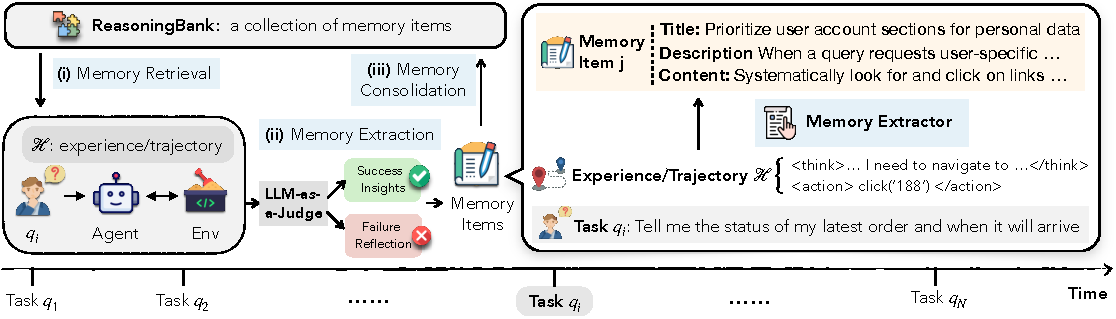
\includegraphics[width=\textwidth]{figures/ReasoningBank.pdf}
\end{center}
% \vspace{-5mm}
\caption{Overview of \ours{}. Experiences are distilled into structured memory items with a title, description, and content. For each new task, the agent retrieves relevant items to interact with the environment and constructs new ones from both successful and failed trajectories, using LLM-as-a-Judge as a signal provider. These items are then consolidated into \ours{}, forming a closed-loop memory process.}
\label{fig: reasoningbank}
% \vspace{-5mm}
\end{figure}

\subsection{\ours{}}\label{sec: reasoningbank}

Past raw trajectories (or experiences), while being comprehensive and original, are often too lengthy and noisy to be directly applied to the current user query. As illustrated in Figure~\ref{fig: reasoningbank}, \ours{} distills useful strategies and reasoning hints from past experiences into structured memory items, which are then stored in the agent’s memory for future reuse.

\noindent\textbf{Memory Schema.} Memory items in \ours{} are designed and induced from past experiences as structured knowledge units that abstract away low-level execution details while preserving transferrable reasoning patterns and strategies. 
Each memory item specifies three components: 
(i) a \textit{title}, which serves as a concise identifier summarizing the core strategy or reasoning pattern; 
(ii) a \textit{description}, which provides a brief one-sentence summary of the memory item; and 
(iii) the \textit{content}, which records the distilled reasoning steps, decision rationales, or operational insights extracted from past experiences. 
Together, memory items extracted are both human-interpretable and machine-usable, facilitating efficient usage and integration with agents.

\noindent\textbf{Integrating \ours{} with Agents.} 
An agent $\pi_{\mathcal{L}}$ equipped with \ours{} can draw upon a curated pool of transferable strategies to guide decision-making. This enables the agent to recall effective insights, avoid previously observed pitfalls, and adapt more robustly to unseen queries. 
The integration proceeds in three steps: (i) \textit{memory retrieval}, (ii) \textit{memory extraction}, and (iii) \textit{memory consolidation}, as shown in Figure~\ref{fig: reasoningbank}.
During \textit{memory retrieval}, the agent queries \ours{} with the current query context to identify the top-$k$ relevant experiences and their corresponding memory items using embedding-based similarity search. Retrieved items are injected into the agent’s system instruction, ensuring that action prediction from $\mathcal{A}$ is grounded with useful past experiences.
When the current query task is completed, we will perform \textit{memory extraction} to extract new memory items. The first step is to obtain proxy correctness signals for trajectories: we adopt an LLM-as-a-judge~\citep{gu2024survey} to label outcomes as success or failure given the query and trajectory without any ground-truth reference. Based on these signals, we apply different extraction strategies: successful experiences contribute validated strategies, while failed ones supply counterfactual signals and pitfalls that help sharpen guardrails. In practice, we extract multiple memory items for each trajectory/experience as detailed in Appendix~\ref{app: prompt}.
Finally, \textit{memory consolidation} incorporates these items into \ours{} with a simple addition operation, maintaining an evolving repository of memory items. Details are in Appendix~\ref{app: tech_details}.
Together, these steps form a closed-loop process: the agent leverages past experiences, constructs new memory from current tasks, and continually updates its memory, enabling sustained evolvement in test-time learning scenarios.\footnote{We deliberately keep the memory usage pipeline simple, avoiding additional complexity in retrieval or consolidation so as to highlight the contribution of \ours{} itself. These components, however, can be further enhanced with more sophisticated techniques, which could provide additional benefits.}


\subsection{\mats{}: Memory-aware Test-Time Scaling}\label{sec: tts}

\ours{} enables learning from experiences to translate more experiences into greater improvements.
As test-time scaling~\citep{snell2025scaling} recently emerged as a powerful strategy for boosting the performance of LLM agents~\citep{zhu2025scaling}, it shows strong potential by allocating additional inference-time computation to generate abundant exploration histories.
A direct combination of \ours and test-time scaling is depicted in Figure~\ref{fig: mats}(a), where more trajectories are independently converted to more memory items.
However, this vanilla form is suboptimal because it does not leverage inherent contrastive signal that arises from redundant exploration on the same problem, which limits the resulting performance advantage brought by test-time scaling.
To address this, we propose \textit{Memory-aware Test-Time Scaling} (\mats{}), a novel integration of test-time scaling with \ours{}. Unlike the vanilla approach, \mats{} deliberately learns from the abundant successful and failure trajectories generated during scaling for more effective memory curation.
We design two complementary instantiations for \mats{}, parallel scaling and sequential scaling, as illustrated in Figure~\ref{fig: mats}(b) and \ref{fig: mats}(c) with detailed implementation in Appendix~\ref{app: prompt_mats}.

\begin{figure}[t]
\begin{center}
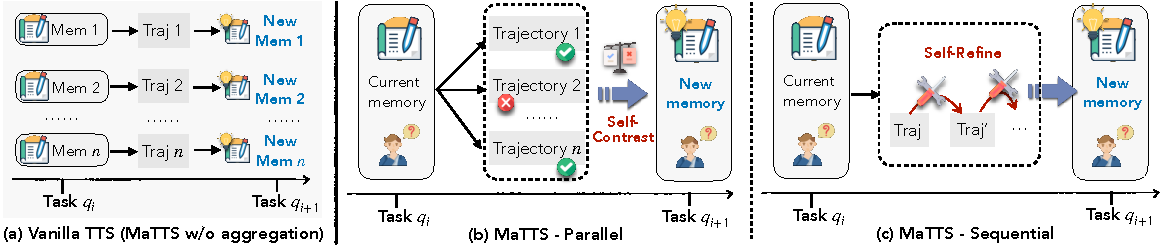
\includegraphics[width=\textwidth]{figures/matts.pdf}
\end{center}
% \vspace{-5mm}
\caption{Comparison of \textit{(a) vanilla TTS} and \mats{} with \textit{(b) parallel scaling}, where self-contrast across multiple trajectories curates reliable memory, and \textit{(c) sequential scaling}, where self-refinement enriches memory with intermediate reasoning signals.}
\label{fig: mats}
% \vspace{-5mm}
\end{figure}

\noindent\textbf{Parallel Scaling.} 
In the parallel setting, we generate multiple trajectories for the same query under the guidance of retrieved memory items. 
By comparing and contrasting (\textit{self-contrast}~\citep{chen2020simple}) \textit{across different trajectories}, the agent can identify consistent reasoning patterns while filtering out spurious solutions. 
This process enables more reliable memory curation from multiple trials of a single query that promotes diverse exploration. 

\noindent\textbf{Sequential Scaling.} 
We iteratively refines its reasoning \textit{within a single trajectory} after the initial completion, following the principle of \textit{self-refinement}~\citep{madaan2023self}. 
During this process, the intermediate notes generated in self-refinement are also used as valuable signals for memory, since they capture reasoning attempts, corrections, and insights that may not appear in the final solution. 

We define the scaling factor $k$, denoting the number of trajectories for parallel scaling and refinement steps for sequential scaling. Equipped with \ours{}, both parallel and sequential strategies become memory-aware, ensuring that the additional computation allocated at test time translates into more transferable and higher-quality memory for future tasks.
